\documentclass[12pt,a4paper,titlepage]{report}
\usepackage[utf8]{inputenc}
\usepackage[francais]{babel}
\usepackage{amsmath}
\usepackage{amsfonts}
\usepackage{amssymb}
\usepackage{graphicx}
\usepackage{url}
\usepackage{hyperref}
\usepackage[hyphenbreaks]{breakurl}
\urlstyle{same}
\hypersetup{ %
colorlinks=false %
,hidelinks %
}


% Police Times
\usepackage{times}

% Mise en forme des tableaux
\usepackage{longtable}
\usepackage{array}
\usepackage{footnote}

% Definition de l'affichage du code
\usepackage{listingsutf8}
\lstset{basicstyle=\footnotesize\ttfamily
%,frame=single
,showstringspaces=false
,tabsize=3
 ,escapeinside={\%*}{*)}
,breaklines=true
,inputencoding=utf8
}
%,extendedchars=false
%,escapeinside=~
% ,inputencoding=latin1
%inputencoding=utf8/latin1
%,backgroundcolor=\color{lightgray}
%,numbers=left
\author{Eric Quinton}
\title{Collec : description des services web}
\date{\today -- v0.1}

%Supprime les veuves et orphelines
\widowpenalty=10000
\clubpenalty=10000
\raggedbottom 
\begin{document}
\maketitle
\chapter{Le logiciel Collec-Science}
\section{Historique}

L'unité de recherche \textit{Écosystèmes aquatiques et changements globaux} d'IRSTEA, à Cestas (33), récolte et manipule des échantillons prélevés sur le terrain (ou plutôt, principalement dans l'eau -- estuaires, lacs, rivières...), et les stocke, parfois pour des durées très longues : certaines campagnes de collecte ont eu lieu il y a plus de 40 ans.

De plus en plus, des échantillons anciens sont réanalysés (analyses génétiques, étude des ossements des oreilles ou otolithes...), au gré des questions scientifiques à traiter. 
Le besoin de recourir à un logiciel pour gérer ces matériels est devenu une priorité.

Dans un premier temps, quelques logiciels open-source susceptibles d'être utilisés ont été étudiés. Toutefois, leurs limites sont vite apparues : problème de pérennité, ancienneté du code, modèle de distribution parfois insatisfaisant (une licence open-source est obligatoire pour assurer la pérennité à longue échéance), résistance aux attaques informatiques, fonctionnalités insuffisantes ou inadaptées au besoin.

Dans un second temps, une étude des besoins réels a été menée. De nouvelles fonctionnalités ont été rajoutées, comme la gestion du stock de matériel utilisé sur le terrain, stocké dans un hangar.

L'unité de recherche s'intégrant au niveau régional avec d'autres organismes, des collaborations avec l'Observatoire Aquitain des Sciences de l'Univers (OASU) ou l'université de La Rochelle ont été envisagées.
Des échanges productifs ont ainsi pu être mis en place, entre autres sur la gestion de l'étiquetage et le scannage des codes-barres.

Le logiciel a largement évolué suite à ces échanges, de nombreuses fonctionnalités ont été rajoutées ou modifiées pour tenir compte des besoin des partenaires potentiels. 

Les délais de développement de la première version opérationnelle se sont étalés sur 9 mois, entre la définition des besoins et le développement proprement dit. 
La première version est parue à l'automne 2016, la version 2.0 est sortie en mai 2018.

Le code comprend environ 15800 lignes (commentaires compris), dont 7600 concernent l'affichage des pages web. Il a été écrit en PHP, les pages web sont générées en HTML et Javascript avec le composant Smarty.

\section{Fonctionnalités générales}

\begin{figure}[H]
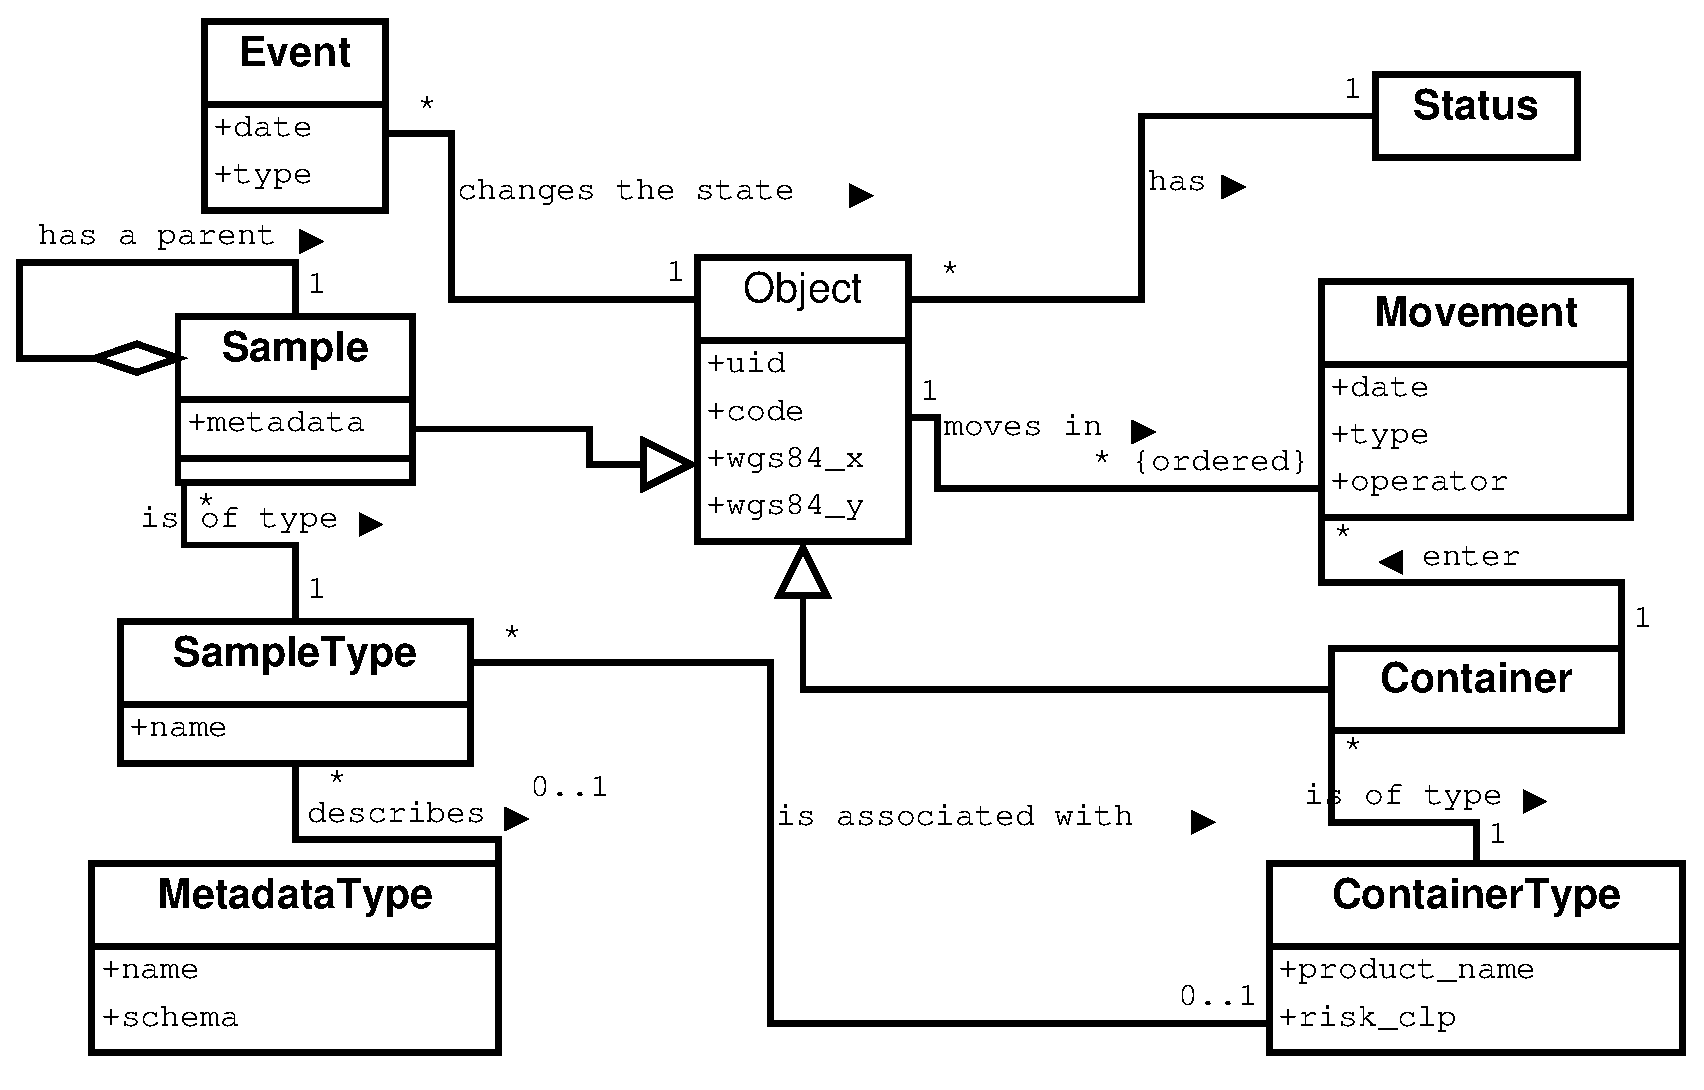
\includegraphics[width=\linewidth]{images/classes2}
\caption{Représentation objet de la base de données}
\end{figure}


Deux types d'objets sont manipulés dans l'application :
\begin{itemize}
\item des conteneurs (container), qui peuvent contenir des objets de tout type : d'autres conteneurs ou des échantillons. Ils peuvent être de différentes nature : site, bâtiment, salle, armoire, caisse, éprouvette... Les types de conteneurs décrivent également le produit de conservation utilisé et le risque associé (brûlure, cancérogène, etc.) ;
\item des échantillons (sample), qui peuvent être associés à un type de conteneur : il y a de nombreux cas où l'échantillon lui-même se confond avec son contenant, par exemple quand le résultat d'une pêche n'est pas trié et est stocké dans un bocal.
\end{itemize}

Un échantillon ou un conteneur sont issus d'un objet unique, qui est doté :
\begin{itemize}
\item d'un numéro unique, l'\textbf{UID}, qui sert de référence dans le logiciel ;
\item d'un identifiant métier, qui servira à le retrouver facilement (le logiciel permet également de définir d'autres identifiants).
\end{itemize}

Un objet peut subir un certain nombre d'événements, voire être réservé (fonctionnalité très simplifiée, seul le recouvrement de deux périodes de réservation est signalé).

Tout objet peut être étiqueté. Les étiquettes peuvent comprendre un code-barre 2D de type QRCode, qui pourra être lu soit à partir d'un terminal dédié (douchette), soit avec une tablette ou un smartphone, l'application disposant d'un module capable d'activer la caméra depuis le navigateur et de scanner le code-barre.

Un échantillon est obligatoirement rattaché à une collection. Seuls les les personnes rattachées à celle-ci peuvent modifier les informations le concernant. 

Pour mieux décrire les échantillons, il est possible de leur rattacher quelques informations \og métier \fg{}, appelées ici \textit{métadonnées}. Les types de métadonnées, totalement paramétrables, sont rattachés aux types d'échantillons.

Un échantillon peut être subdivisé en d'autres échantillons. Par exemple, des otolithes (os de l'oreille) peuvent être extraits d'un poisson. Le logiciel permet de créer un nouvel échantillon à partir d'un autre, qui peut être d'un autre type le cas échéant, et qui restera associé au parent. 

Enfin, dans certains cas de figures, un échantillon peut être composé de plusieurs éléments indifférenciés, par exemple plusieurs écailles de poisson prélevées et conservées ensemble. Le logiciel permet d'indiquer les prélèvements et les restitutions réalisées, et affiche le solde (théorique !) restant.

\section{Technologie employée}
\subsection{Base de données}

L'application a été conçue pour fonctionner avec Postgresql, en version 9.5. Les versions antérieures peuvent être utilisées, mais seule cette version dispose d'un type de données JSON qui permet de stocker les informations métiers.

\subsection{Langage de développement et framework utilisé}
Le logiciel a été écrit en PHP, en s'appuyant sur le framework \textit{Prototypephp} \cite{prototypephp}, développé parallèlement par l'auteur du logiciel.

Il utilise la classe \textit{Smarty} \cite{smarty} pour gérer l'affichage des pages HTML. Celles-ci sont générées en utilisant \textit{Jquery} \cite{jquery}  et divers composants associés. Le rendu général est réalisé avec \textit{Bootstrap} \cite{bootstrap}.

Les étiquettes sont générées en utilisant FOP \cite{fop}, une classe Java qui crée des fichiers PDF à partir d'un fichier XML contenant les données et un fichier de transformation au format XSL.

\subsection{Liste des composants externes utilisés}

\begin{longtable}{|>{\raggedright\arraybackslash}p{3cm}|c|c|>{\raggedright\arraybackslash}p{3cm}|>{\raggedright\arraybackslash}p{3cm}|}
\hline 
\textbf{Nom} & \textbf{Version} & \textbf{Licence} & \textbf{Usage} & \textbf{Site} \\ 
\hline 
\endhead
PrototypePHP & branche bootstrap & LGPL & Framework & \href{https://github.com/equinton/prototypephp}{github.com/ equinton/ prototypephp} \\ 
Smarty & 3.1.31 & LGPL & Générateur de pages HTML & \href{http://www.smarty.net}{www.smarty.net} \\ 
Smarty-gettext & 1.2.0 & LGPL & Support multi-langues pour Smarty & \\
PHPCAS & 1.3.5 & Apache 2.0 & Identification auprès d'un serveur CAS & \href{https://wiki.jasig.org/display/CASC/phpCAS}{wiki.jasig.org/ display/ CASC/ phpCAS} \\ 
PHPQRCODE &  1.1.4 & LGPL & Génération des qrcodes & \\
Zxcvbn-PHP & 0.3 & MIT & Vérification de la complexité des mots de passe & \\

\hline 
\caption{Table des composants PHP externes utilisés dans l'application}
\end{longtable} 

\begin{longtable}{|>{\raggedright\arraybackslash}p{3cm}|c|c|>{\raggedright\arraybackslash}p{3cm}|>{\raggedright\arraybackslash}p{3cm}|}
\hline 
\textbf{Nom} & \textbf{Version} & \textbf{Licence} & \textbf{Usage} & \textbf{Site} \\ 
\hline 
\endhead
Bootstrap & 3.0 & MIT & Présentation HTML & \href{http://getbootstrap.com}{get.bootstrap.com} \\ 
ComboBox & 1.0.1 & MIT & gestion des combobox & \\

JavaScript Cookie & 2.1.4 & MIT & Gestion des cookies dans le navigateur & \href{https://github.com/js-cookie/js-cookie}{github.com/ js-cookie/ js-cookie} \\ 

Datatables & 1.10.20 & MIT & Affichage des tableaux HTML & \href{http://www.datatables.net/}{www.datatables. net} \\ 

Datetime-moment &  & MIT & Formatage des dates dans les tableaux & \href{https://datatables.net/plug-ins/sorting/datetime-moment}{datatables.net/ plug-ins/ sorting/ datetime-moment} \\ 

Moment &  & MIT & Composant utilisé par datetime-moment & \href{http://momentjs.com} {momentjs.com}\\ 

JQuery & 3.3.1 & $\approx$ BSD & Commandes Javascript & \href{http://jquery.com/}{jquery.com} \\ 

JQuery-ui & 1.12.1 & $\approx$ BSD & Commandes Javascript pour les rendus graphiques & \href{http://jqueryui.com/}{jqueryui.com} \\ 

js.cookies & 0.0.4 & & Gestion des cookies & \\

leaflet & 1.3.4 & & Affichage des cartes OpenStreetMap & \\
leaflet-draw & 1.0.4 & & Dessin de polygones sur les cartes & \\
leaflet-mouse-position & 1.2.0 & & récupération de la position de la souris & \\
leaflet-marker-cluster & 1.4.1 & & & \\
leaflet-tylelayer-pouchdbcached & 1.0.0 & & Mise en cache de la cartographie & \\
pouchdb & 7.1.1 & & moteur de mise en cache & \\

Jquery-timepicker-addon &  & MIT & Time picker & \href{https://github.com/trentrichardson/jQuery-Timepicker-Addon}{github.com/ trentrichardson/ jQuery-Timepicker-Addon} \\ 

Magnific-popup & 1.1.0 & MIT & Affichage des photos & \href{http://dimsemenov.com/plugins/magnific-popup/}{dimsemenov .com/plugins/ magnific-popup/}\\ 

Smartmenus & 1.1.0 & MIT & Génération du menu HTML & \href{http://www.smartmenus .org}{www.smartmenus .org} \\ 
 
Openlayers & 4.2.0 & BSD & Affichage des cartes & \href{http://openlayers.org/}{openlayers.org} \\ 

qcode-decoder & & MIT & lecture de codes barres & \href{http://cirocosta.github.io/qcode-decoder/}{cirocosta.github .io/qcode-decoder}\\

Html5-qrcode &  & MIT & Lecture des QRcodes &  \href{https://github.com/dwa012/html5-qrcode}{github.com/ dwa012/ html5-qrcode} \\ 

AlpacaJS & 1.5.23 & Apache 2 & Génération et saisie des métadonnées & 
\href{http://www.alpacajs.org/}{www.alpacajs.org}\\

handlebars & 4.5.3 & & Gestion des boutons dans AlpacaJS & \\
zxcvbn & 4.4.2 & & Vérification de la complexité des mots de passe & \\
\hline
\caption{Table des composants Javascript externes utilisés dans l'application}
\end{longtable} 

\section{Sécurité}

L'application a été conçue pour résister aux attaques dites opportunistes selon la nomenclature ASVS v3 \cite{asvs} de l'OWASP \cite{owasp}. Des tests d'attaque ont été réalisés en août 2016 avec le logiciel ZAProxy \cite{zaproxy}, et n'ont pas détecté de faiblesse particulière.

La gestion des droits est conçue pour :
\begin{itemize}
\item qu'un utilisateur, membre d'une collection, ne puisse modifier que les échantillons qui y sont rattachés ;
\item que tout utilisateur disposant des droits de gestion peut procéder à une entrée ou une sortie d'un objet, quel qu'il soit ;
\item que les responsables d'une collection soient les seuls à pouvoir modifier les paramètres comme les types d'échantillons ou de conteneurs, les protocoles ou les opérations rattachées.
\end{itemize}
L'analyse de sécurité a mis en exergue un besoin de ne pas perdre d'information : si un échantillon est étiqueté et rangé, et que l'information est perdue, il y a de gros risques de ne plus pouvoir l'utiliser ultérieurement. Cela impose la mise en place d'un mécanisme de réplication de la base de données, à implémenter -- ou faire implémenter par des administrateurs du système -- directement dans Postgresql.

\section{Licence}
Le logiciel est diffusé selon les termes de la licence GNU AFFERO GENERAL PUBLIC LICENSE version 3, en date du 19 novembre 2007 \cite{agpl}.

\section{Copyright}

L'application a été déposée par IRSTEA auprès de l'Agence de protection des programmes \cite{app}, sous le numéro IDDN.FR.001.470013.000.S.C.2016.000.31500


\chapter{Gestion des habilitations -- principes retenus pour le logiciel Collec}
\label{oauth}

Le mécanisme d'identification prévu pour les services web s'appuie en grande partie sur le protocole OAuth v2, au moins dans ses principes. Ce n'est pas le protocole qui est effectivement implémenté (OAuth est prévu pour que l'utilisateur définisse les droits d'accès de l'application cliente), mais les principes d'identification retenus s'en inspirent.

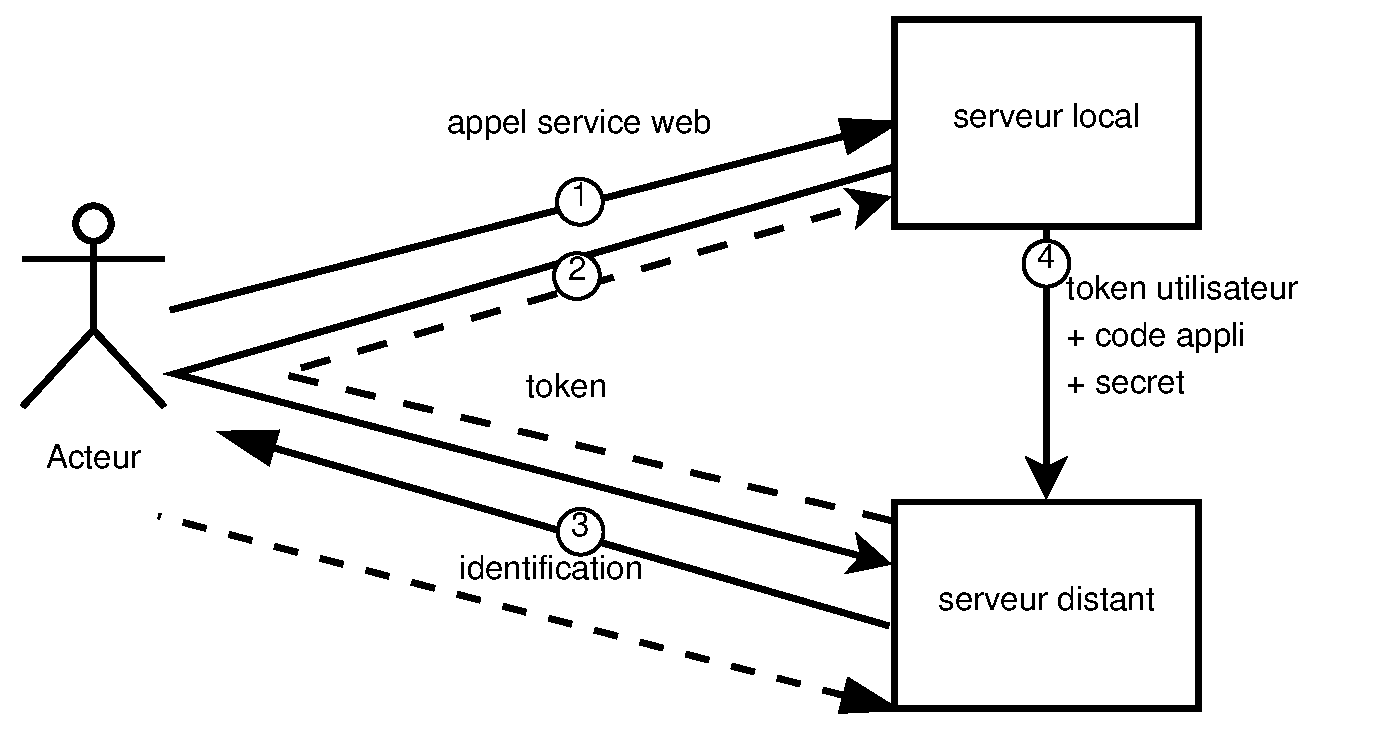
\includegraphics[width=\linewidth]{images/appel_sw_identification}

Pour accéder à des informations distantes, le dialogue entre les deux serveurs nécessite plusieurs phases :
\begin{enumerate}
\item l'utilisateur veut déclencher l'appel à un service web distant ;
\item aucun jeton n'a été récupéré par le serveur local : l'utilisateur est redirigé vers le serveur distant pour obtenir un jeton d'identification;
\item le serveur distant ne connaît pas l'utilisateur : il lui demande de s'identifier en utilisant la procédure adéquate (\textit{login/mot de passe} dans la plupart des cas);
\\une fois identifié, le serveur distant renvoie le navigateur de l'utilisateur vers le serveur local, en fournissant un jeton chiffré;
\item l'appel au service web peut maintenant être déclenché, en fournissant:
\begin{itemize}
\item le jeton de l'utilisateur;
\item le code de l'application locale;
\item le secret partagé entre l'application distante et l'application locale.
\end{itemize}
\end{enumerate}


\section{Opérations préalables à l'interrogation d'une \\base de données distante}
\subsection{Identification réciproque des applications}

Les applications clientes doivent se faire identifier par les applications distantes avant tout échange.

Cette étape est manuelle : l'administrateur de l'application distante crée un enregistrement dans la table \textit{instance}, dont le détail est décrit dans la section \ref{table_instance}.

Le code d'identification, ainsi que le secret associé, est envoyé par mail (de manière automatique ou semi-automatique de préférence) par l'administrateur de la base distante (\textit{cf.} section \ref{dist_record}).

Ces informations sont stockées dans la table \textit{instance} locale, en indiquant en outre les adresses des différents services web disponibles pour le serveur distant.

\subsection{Identification des utilisateurs}
Les utilisateurs qui peuvent utiliser les services web distants sont enregistrés dans le serveur distant et disposent d'un code d'identification. Une fois connectés, ils doivent hériter du droit \textit{consultsw}, indispensable pour accéder aux services web.

Pour qu'ils puissent récupérer les données \og métier \fg{}, les utilisateurs doivent également être rattachés à un projet. Dans la pratique, dans la gestion des groupes de logins, on trouvera l'arborescence suivante (par exemple):
\begin{center}

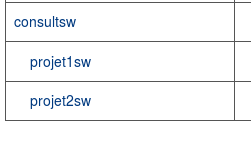
\includegraphics[width=5cm]{images/arborescence_groupes_sw}

\end{center}

Les utilisateurs distants sont associés aux groupes \textit{projet1sw} ou \textit{projet2sw}, et ces groupes sont associés aux projets (ou sous-collections) adéquats pour leur donner les droits d'accès en lecture.

\chapter{Description des services web}

\section{Remarques générales}

Les services web sont destinés à fournir des informations aux clients. Leur implémentation dépend des logiciels, ainsi que la manière de traiter les données.

Pour des raisons de compatibilité entre les différents logiciels, si un argument fourni figure dans la requête mais n'est pas utilisable par le service web, ce dernier ne doit pas rejeter la requête, sauf si aucun argument ne permet de discriminer la recherche demandée.

\subsection{Format des données transmises ou reçues}
Les données sont échangées au format JSON.

Les requêtes sont de type GET\footnote{Les requêtes de type POST sont prévues pour créer un enregistrement, PUT pour mettre à jour une partie d'un enregistrement, DELETE pour le supprimer.}. 
Actuellement, aucun service web n'est prévu pour mettre à jour des informations dans la base distante.

\subsection{Codes d'erreur}

Voici la liste minimale des codes d'erreur génériques que les services web devraient retourner :
\begin{longtable}{|c|>{\raggedright\arraybackslash}p{10cm}|}
\hline 
Code &  Description \\ 
\hline \endhead
400 & Bad argument : un des arguments fournis n'est pas valide, ou aucun argument utilisable n'a été indiqué\footnote{Dans le cas où des arguments sont fournis, mais non utilisables par le service web considéré, l'exécution de la requête conduisant à renvoyer trop d'informations} \\
\hline
401 & Unauthorized : les droits d'accès sont insuffisants pour permettre d'obtenir les informations \\
\hline
404 & Not found : la ressource demandée est introuvable\\
\hline
408 & RequestTimeOut : la requête n'a pas abouti dans le temps imparti, ou elle a été annulée par le client\\
\hline
500 & InternalError : une erreur d'exécution ne permet pas de retourner le résultat de la requête\\
\hline
503 & ServiceUnavailable : le service est temporairement indisponible\\
\hline
\end{longtable} 

\section{Table des listes techniques}

Ce service web permet de récupérer la liste des tables de référence qui peuvent être utilisées pour lancer une recherche.

\subsection{url type}
\url{https://sitedistant.fr/sw/v1/params}

\subsection{Données en entrée}
Le service web ne nécessite pas de paramètre d'entrée.


\subsection{Données en retour}
La requête retourne la liste demandée sous la forme d'une collection Json contenant les informations suivantes :

\begin{longtable}{|c|c|>{\raggedright\arraybackslash}p{6cm}|}
\hline 
Code & Type & Description \\ 
\hline
code & varchar & Code de la table de référence. C'est ce code qui sera utilisé pour obtenir la liste des valeurs disponibles dans le service web de récupération du contenu\\
\hline
val & varchar & Texte affichable dans un masque de recherche\\
\hline
valfr & varchar & Texte affichable dans un masque de recherche, en français\\
\hline
valen & varchar & Texte affichable dans un masque de recherche, en anglais\\
\hline \endhead
\end{longtable}

Exemple :
\begin{lstlisting}
[
{code:"project",val:"Projets", valen:"projects"},
{code:"sampletype",val:"Types d'echantillons", valen:"samples types"},
{code:"identifiertype",val:"Identifiants metier", valen:"business identifiers"},
{code:"place",val:"Lieux de prelevement des echantillons",valen:"sampling places"}
]
\end{lstlisting}

\section{Listes techniques}
\label{listes}

Ce service web permet de récupérer une liste de référence nécessaire pour comprendre ou rechercher les échantillons de la base distante.

\subsection{url type}
\url{https://sitedistant.fr/sw/v1/reference/project} ou 
\url{https://sitedistant.fr/sw/v1/reference/var=project}.

La valeur fournie (\textit{project} ici) est une des valeurs récupérée dans le service web précédent (rubrique \textit{code}).

La requête est de type GET. 


\subsection{Données en retour}
La requête retourne la liste demandée sous la forme d'une collection Json contenant les informations suivantes :

\begin{longtable}{|c|c|>{\raggedright\arraybackslash}p{10cm}|}
\hline 
Code & Type & Description \\ 
\hline
id & integer & Identifiant interne\\
\hline
val & varchar & Libellé\\
\hline
comment & varchar & Description ou commentaire\\
\hline \endhead
\end{longtable}

Exemple :
\begin{lstlisting}
[
{id:1,val:"projet1",comment:"Description du projet 1"},
{id:3,val:"projet3",comment:"Descripton du projet 3"}
]
\end{lstlisting}


\section{Rechercher des échantillons}
\label{sampleSearch}
\subsection{url type}
\url{https://sitedistant.fr/sw/v1/sample_search?param={uidstart:10,uidend:15}}

\url{https://sitedistant.fr/sw/v1/sample_search?uidstart=10&uidend=15}

\subsection{Variables de recherche}
Les variables sont fournies soit dans la requête GET, soit sous la forme d'une variable JSON nommée \textit{param}.

% \usepackage{array} is required
\begin{longtable}{|c|c|>{\raggedright\arraybackslash}p{8cm}|}
\hline 
Code & Type & Description \\ 
\hline \endhead
\hline \endfoot
uid & integer & Identifiant unique de l'échantillon dans l'instance distante \\ 
\hline 
ident & varchar & identifiant \og métier\fg{} principal \\
\hline
guid & UUID & identifiant unique quel que soit la base de données \\
\hline
uidstart & integer & uid inférieur pour une recherche sur une fourchette d'identifiants \\
\hline
uidend & integer & uid supérieur pour une recherche sur une fourchette d'identifiants \\
\hline
datestart & yyyy-mm-dd & date de début pour une recherche sur une fourchette de dates \\
\hline
dateend & yyyy-mm-dd & date de fin pour une recherche sur une fourchette de dates \\
\hline
codefamily & objet Json & objet json permettant de rechercher une valeur sur une table de paramètres. \textit{Codefamily} doit être remplacé par le code retourné lors de la recherche des listes de paramètres. \\
& & L'objet JSON accepte, comme informations associées : \\
& & \textit{id} : identifiant spécifique à rechercher (par exemple, le code de l'identifiant métier). \textit{id} peut être facultatif, si la recherche ne porte que sur la valeur, par exemple, le lieu de prélèvement; \\
& & \textit{val} : valeur recherchée\\
& & si uniquement \textit{val} est indiqué, on peut utiliser un couple classique: \textit{codefamily:val}\\
\hline
\end{longtable} 

Exemple de contenu pour la variable \textit{\$param} : 
\begin{lstlisting}
{"uidstart": 25,
"uidend": 50,
"datestart": "2017-01-01",
"dateend": "2017-06-30",
"identifiertype":{"id":10, "val":"AB01"},
"sampletype":2
}
\end{lstlisting}

La recherche portera sur les échantillons dont l'UID est entre 25 et 50, dont la date est entre le 1\ier{} janvier et le 30 juin 2017, dont l'identifiant métier connu sous le numéro 10 vaut AB01, et dont le type d'échantillons est 2.

\subsection{Données en retour}
Collection Json avec, pour chacun, les informations suivantes :
\begin{longtable}{|c|c|>{\raggedright\arraybackslash}p{6cm}|}
\hline 
Code & Type & Description \\ 
\hline \endhead
uid & integer & Identifiant dans l'instance \\
\hline
identifier & varchar & identifiant principal \og métier\fg{} \\
\hline
guid & uuid & code d'identification global \\
\hline
ids & collection & liste de tous les identifiants secondaires, selon la forme idtype: idval \\
\hline
project & varchar & nom du projet ou de la sous-collection correspondante \\
\hline
createdate & yyyy-mm-dd hh:mm:ss & date de création de l'échantillon dans la base de données d'origine \\
\hline
collectdate & yyyy-mm-dd hh:mm:ss & date de collecte ou de génération de l'échantillon\\
\hline
metadata & objet json & données \og métier\fg{} rattachées à l'échantillon \\
\hline
sampleparent & objet json & json de même structure que ce tableau comprenant les informations du parent (imbrication des différents parents le cas échéant)\\
\hline
storageproduct & varchar & produit de stockage utilisé \\
\hline
clp & varchar & risques associés aux produit de stockage \\
\hline
subsampletype & varchar & type de sous-échantillonnage \\
\hline
subsampleunit & varchar & unité de sous-échantillonnage \\
\hline
subsampleqty & double & quantité de sous-échantillons présents initialement \\
\hline
samplingplacename & varchar & nom du lieu de collecte \\
\hline
\end{longtable}

\section{Lire un échantillon}

\subsection{url type}
\url{https://sitedistant.fr/sw/v1/sample/14}

\url{https://sitedistant.fr/sw/v1/sample?id=TEST-IDENTIFIANT-METIER}

\url{https://sitedistant.fr/sw/v1/sample/guid=e764aca5-75ee-4d23-87a6-78b91202ba37}

\subsection{Variables de recherche}
La requête, de type GET, contient soit en dernière valeur l'UID de l'échantillon à lire, soit une variable GET dont le nom correspond à l'identifiant recherché et la valeur associée
Les valeurs utilisables dans les champs sont les suivants :
\begin{savenotes}
\begin{longtable}{|c|c|>{\raggedright\arraybackslash}p{7cm}|}
\hline 
id & Format attendu dans val & Description \\ 
\hline
uid & integer & Clé utilisée dans la base de données \\
\hline
guid & uuid & Identifiant unique global \\
\hline
id & varchar & Identifiant principal de l'échantillon\\
\hline
xxx & varchar & tout identifiant secondaire disponible
\\
\hline \endhead

\end{longtable}
\end{savenotes}
L'utilisation d'identifiants secondaires n'est pas forcément souhaitable dans tous les cas, notamment si plusieurs échantillons sont susceptibles de présenter le même identifiant secondaire (projets ou sous-collections différents).
\subsection{Données en retour}
Les données en retour sont celles du service de recherche d'un échantillon.

\section{Lire un jeu d'échantillons}
\subsection{url type}
\url{https://sitedistant.fr/sw/v1/samples/{xxx}}

\url{https://sitedistant.fr/sw/v1/samples?param={xxx}}

\subsection{Variables de recherche}
Il s'agit d'une variante du cas précédent. Un fichier JSON est fourni dans la variable \textit{param}, organisé pour fournir un identifiant par échantillon retourné. Voici un exemple du fichier :
\begin{lstlisting}
[{"uid":15},{"id":"A1-B2-C3"}]
\end{lstlisting}
\subsection{Données en retour}
Les données en retour sont celles du service de recherche d'un échantillon.



\chapter{Implémentation technique dans Collec}

\section{Transformation des URL et appel aux modules}
Les URL conviviales sont transformées en noms de modules, selon le fonctionnement suivant :
\begin{itemize}
\item les trois premiers éléments de l'adresse sont fusionnés;
\item si le quatrième élément est présent, il est stocké dans la variable de requête \textit{\$id}, et :
\begin{itemize}
\item si la requête est de type GET, le module est suffixé par \textit{Display};
\item si la requête est de type POST, le module est suffixé par \textit{Write}\footnote{Dans la version actuelle, l'écriture depuis une instance distante n'est pas implémentée};
\end{itemize}
\item sinon, le module est suffixé par \textit{List}.
\end{itemize}

Les modules doivent être décrits, comme les autres, dans le fichier \textit{param/actions.xml}, et sont exécutés selon le fonctionnement classique de l'application.

\section{Emplacement du code}
Le code spécifique des modules doit être stocké dans le dossier \textit{modules}, en respectant l'arborescence des URL conviviales, par exemple, pour l'adresse \textit{http://collec.local/sw/v1/sample}, dans le sous-dossier \textit{sw/v1}.


\subsection{Données d'identification des instances distantes}
\label{table_instance}

Pour identifier les instances clientes, la table \textit{instance} contient les données suivantes :
\begin{itemize}
\item le nom de l'instance;
\item l'url de l'instance ;
\item le nom d'un contact;
\item son mail;
\item le code attribué en conservant les 8 premiers caractères du calcul d'empreintes sha256 de l'url;
\item le secret, généré de manière cryptographique ;
\item le type d'instance (cliente ou serveur);
\item la date de fin d'autorisation d'accès fixée, par défaut, à 5 ans.
\end{itemize}

Si une instance est à la fois cliente et serveur, deux lignes devront être créées, l'une pour chaque sens de communication. Cela permet de maintenir des secrets différents pour chaque canal.

Pour les instances \og serveurs\fg{}, une table complémentaire permet d'indiquer les URI des services web disponibles :
\begin{itemize}
\item le type du service web;
\item l'URI correspondante;
\item mécanisme d'identification.
\end{itemize}

\subsection{Codification des services web}
Afin de permettre les échanges automatisés des paramètres entre les serveurs, le type du service web (son identifiant) doit impérativement respecter le contenu de cette table :
\begin{longtable}{|c|>{\raggedright\arraybackslash}p{10cm}|}
\hline 
Code & Service web  \\ 
\hline \endhead
1 & Liste des tables de paramètres utilisables \\
\hline
2 & Contenu d'une table de paramètres \\
\hline
3 & Recherche d'échantillons \\
\hline
4 & Consultation d'un échantillon \\
\hline
5 & Consultation d'une liste d'échantillons\\
\hline

\end{longtable}

\subsection{Structure des tables correspondantes}

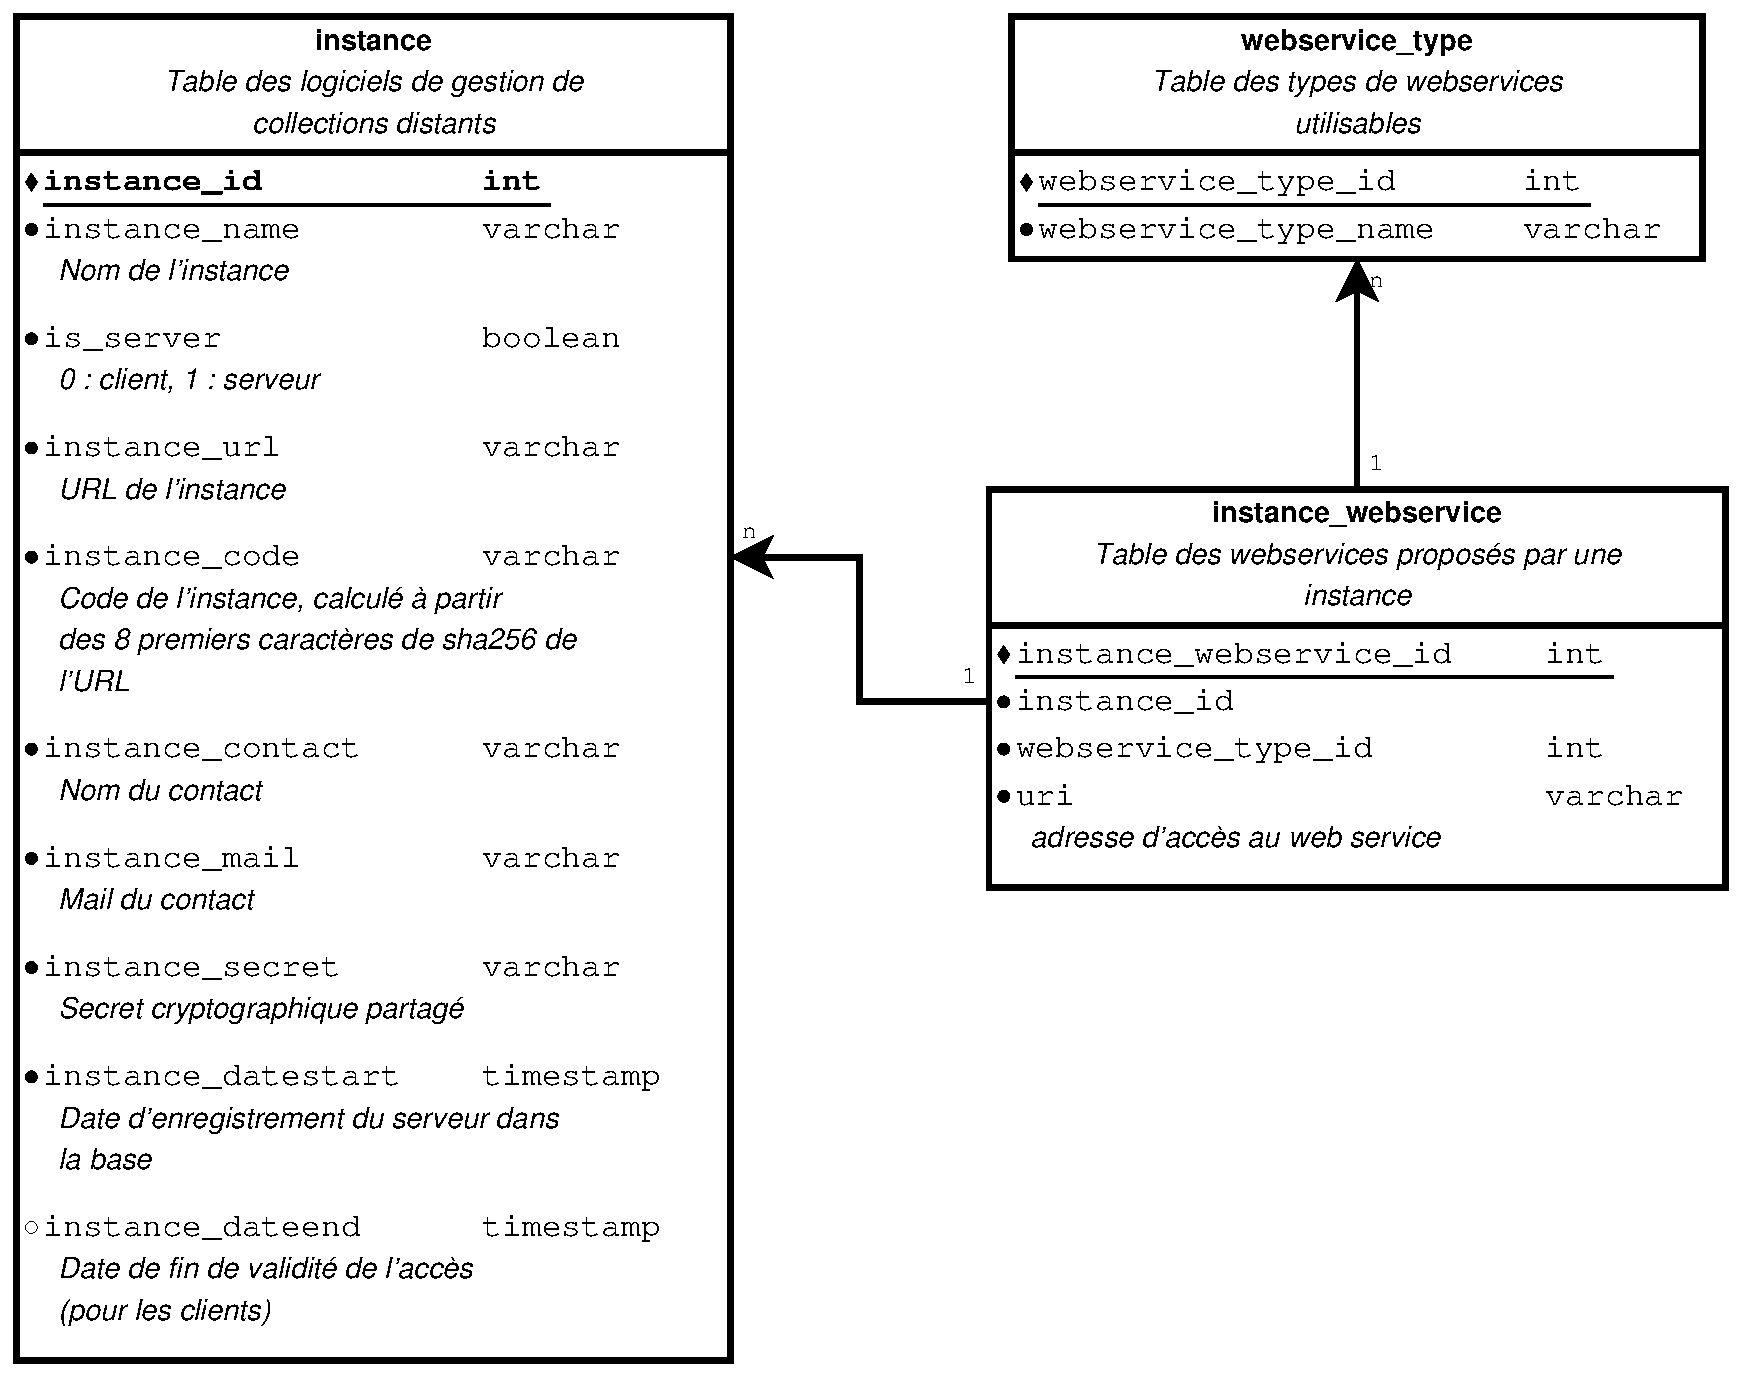
\includegraphics[width=\linewidth]{images/tables_declaration_instances}

\section{Modules et fonctions nécessaires}
\subsection{Enregistrement d'une instance distante cliente}
\label{dist_record}
Ce module doit permettre d'enregistrer les données concernant une instance cliente qui sera autorisée à interroger la base locale. Il faut notamment prévoir :
\begin{itemize}
\item une fonction de génération du secret;
\item le calcul du code de l'instance, basé sur son url;
\item une fonction d'envoi d'un mail au responsable, qui contiendra un fichier json avec les informations suivantes :
\begin{itemize}
\item le code de l'instance;
\item l'url de base;
\item le secret généré;
\item la liste des services web disponibles et l'uri attachée.
\end{itemize}
\end{itemize}

\pagebreak
Voici un exemple de la structure du fichier JSON correspondant :
\begin{lstlisting}
{
"code":"985813d1",
"url":"https://colinstance.irstea.fr",
"secret":"dad90026064f54580d24195acac1f60d2c81426e2efa9719528dee4b0ff13668",
"services":{
	{id:1,"uri":"/sw/v1/params"},
	{id:2,"uri":"/sw/v1/reference"},
	{id:3,"uri":"/sw/v1/sample_search"},
	{id:4,"uri":"/sw/v1/sample"},
	{id:5,"uri":/sw/v1/samples"}
	}
}
\end{lstlisting}

\subsection{Enregistrement d'une instance distante serveur}
Ce module doit faire l'opération inverse de la précédente. Il doit être capable de récupérer le fichier JSON transmis, pour une génération automatique dans la base de données.

\subsection{Identification d'un utilisateur distant}

Un masque de saisie dédié doit être prévu (en cas d'identification via annuaire LDAP ou base de données), pour que l'utilisateur puisse bien confirmer qu'il s'identifie dans un serveur distant.

L'appel doit contenir l'adresse de retour. Le retour doit contenir un jeton, de préférence au format JWT, chiffré avec la clé privée du serveur, avec les informations minimales suivantes :
\begin{itemize}
\item iss : origine (url du serveur);
\item exp: timestamp d'expiration;
\item uid: login de l'utilisateur.
\end{itemize}

\subsection{Module d'interrogation d'un serveur distant}
Le module doit permettre de sélectionner le serveur à interroger. Une fois le serveur sélectionné, la liste des tables de paramètres est récupérée, puis le contenu de ces tables.

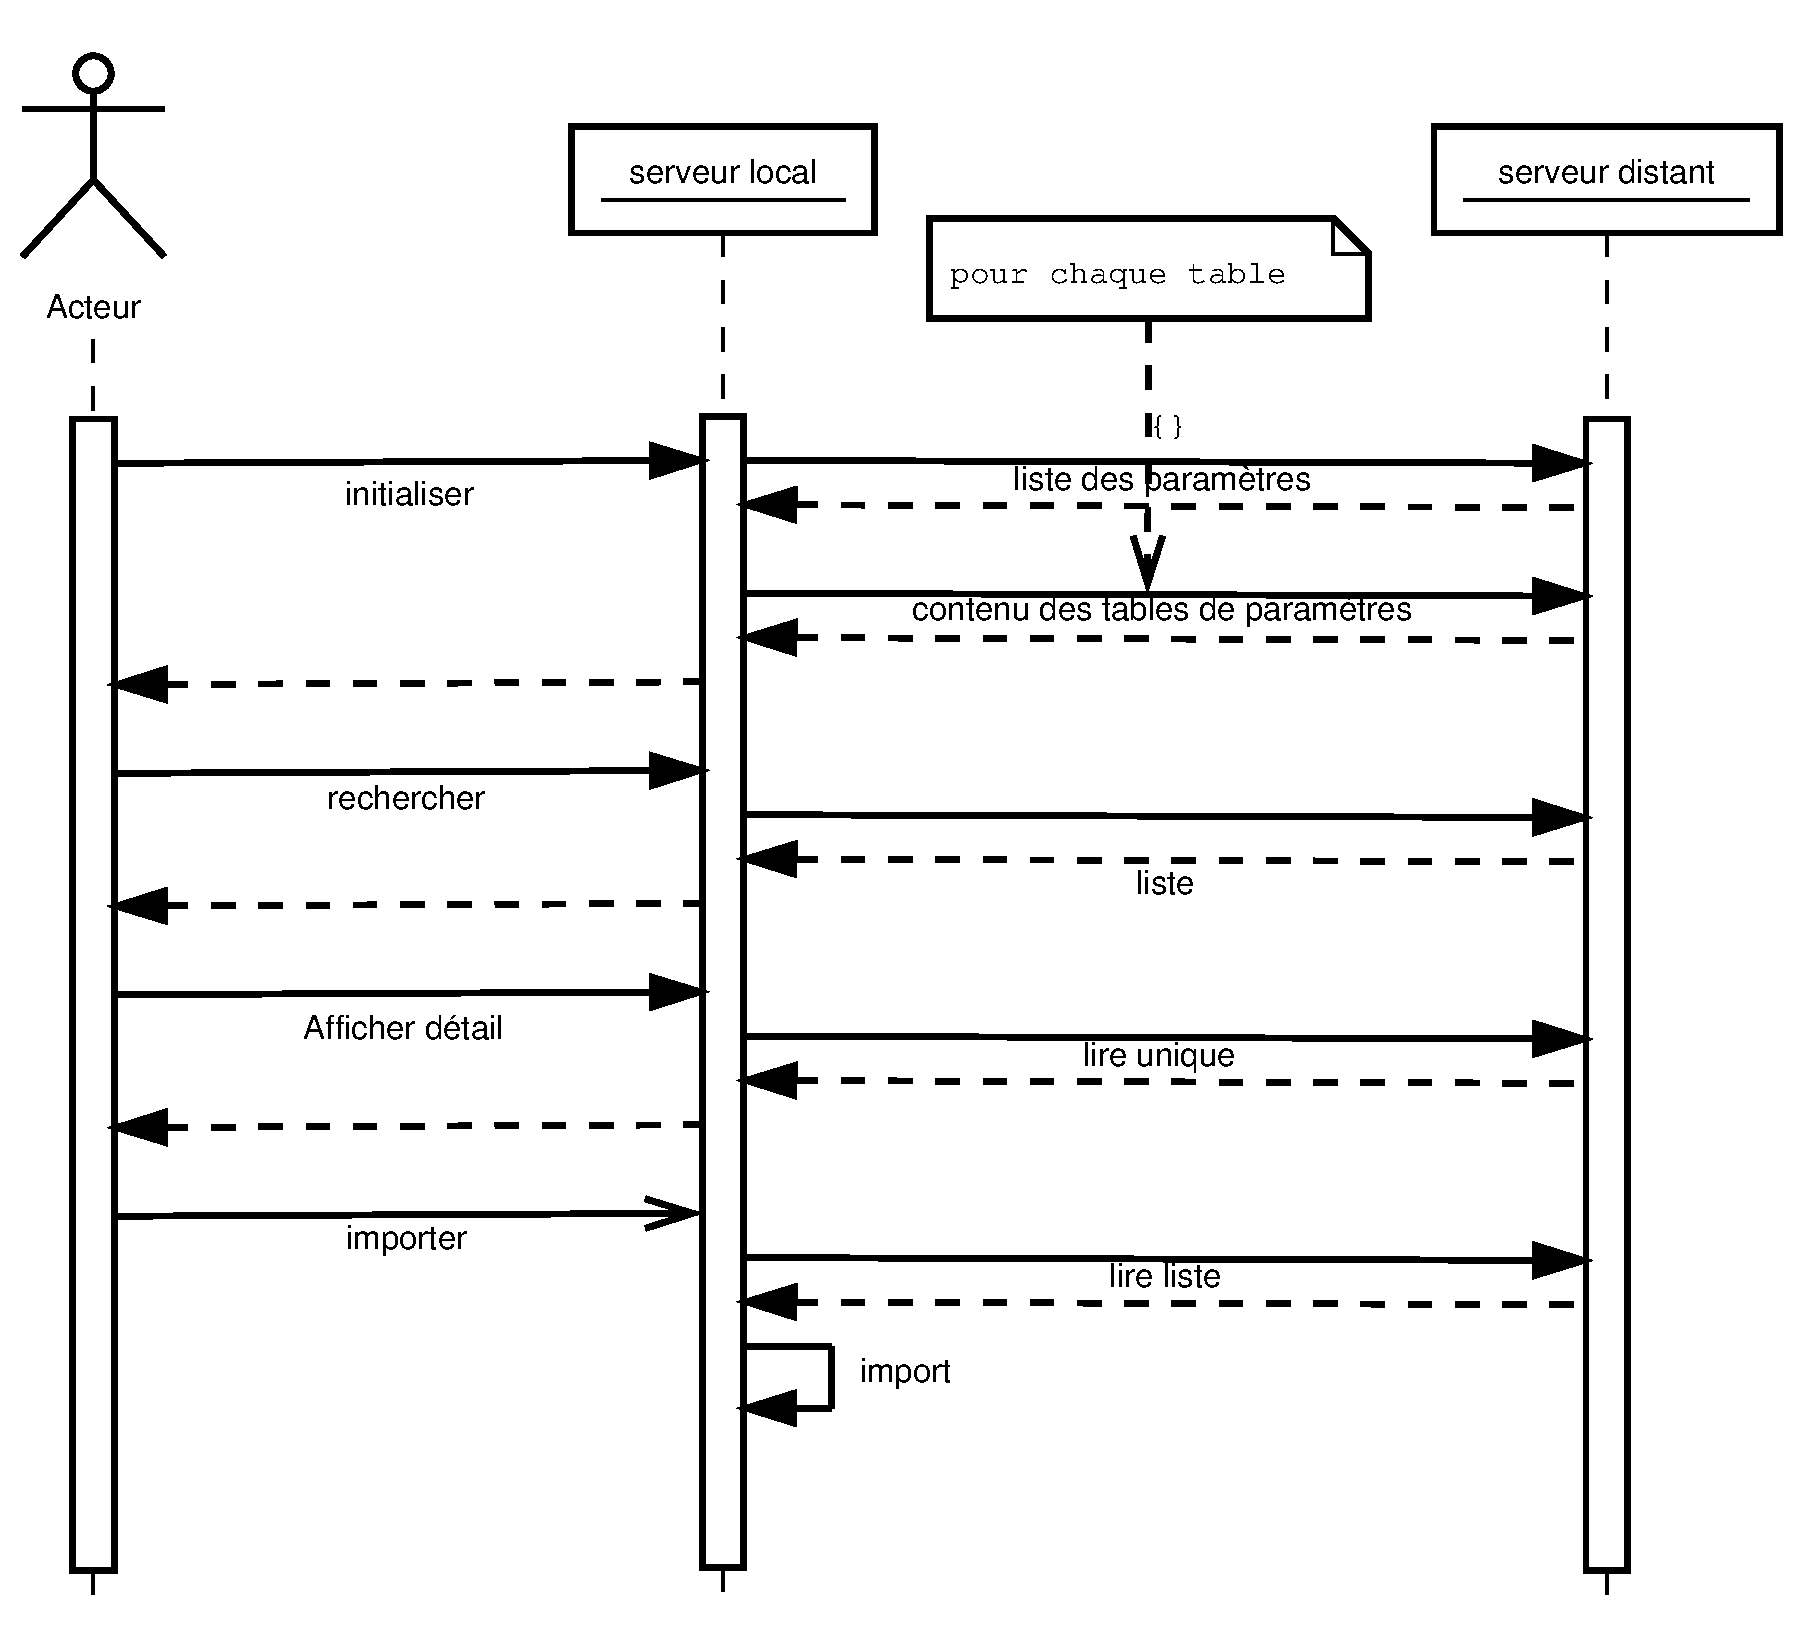
\includegraphics[width=\linewidth]{images/sequence_dans_collec}

Un masque de saisie permet de sélectionner les paramètres de recherche. Une fois les échantillons retrouvés depuis le serveur distant, il doit être possible d'en importer un dans la base locale.

Cet import va passer par une phase intermédiaire pour:
\begin{itemize}
\item associer l'échantillon au type local déclaré;
\item faire la correspondance entre les informations fournies par les tables de paramètres (identifiants secondaires, etc.). Le cas échéant, certaines informations peuvent ne pas être récupérées.
\end{itemize}

L'import ne concerne pas les informations de stockage.


\tableofcontents
\end{document}